\documentclass[twocolumn,english]{IEEEtran}
\usepackage[T1]{fontenc}
\usepackage{babel}
\usepackage{amsthm}
\usepackage{amsmath}
\usepackage{graphicx}
\usepackage[unicode=true,
bookmarks=true,bookmarksnumbered=true,bookmarksopen=true,bookmarksopenlevel=1,
breaklinks=false,pdfborder={0 0 0},backref=false,colorlinks=false]
{hyperref}
\usepackage{bm}
\usepackage{amsmath}
\usepackage{amssymb}
\usepackage{natbib}
\usepackage{siunitx}
\usepackage{array}
\usepackage{calc}
\usepackage{booktabs}
\newcolumntype{W}{>{\centering\arraybackslash}m{25mm}}
\newcolumntype{L}{>{\centering\arraybackslash}m{15mm}}


\hypersetup{
pdftitle=  {Lab 4: Oscillatory Motion},
pdfauthor= {Zack Garza},
pdfpagelayout=OneColumn, pdfnewwindow=true, pdfstartview=XYZ, plainpages=false}

\makeatletter


%%%%%%%%%%%%%%%%%%%%%%%%%%%%%% Textclass specific LaTeX commands.
% protect \markboth against an old bug reintroduced in babel >= 3.8g
\let\oldforeign@language\foreign@language
\DeclareRobustCommand{\foreign@language}[1]{%
  \lowercase{\oldforeign@language{#1}}}
\theoremstyle{plain}
\newtheorem{thm}{\protect\theoremname}
\theoremstyle{plain}
\newtheorem{lem}[thm]{\protect\lemmaname}

%%%%%%%%%%%%%%%%%%%%%%%%%%%%%% User specified LaTeX commands.
% for subfigures/subtables
\ifCLASSOPTIONcompsoc
\usepackage[caption=false,font=normalsize,labelfont=sf,textfont=sf]{subfig}
\else
\usepackage[caption=false,font=footnotesize]{subfig}
\fi

\makeatother
\providecommand{\lemmaname}{Lemma}
\providecommand{\theoremname}{Theorem}
\sisetup{detect-weight=true, detect-family=true}
\setcounter{topnumber}{2}
\setcounter{bottomnumber}{2}
\setcounter{totalnumber}{4}
\renewcommand{\topfraction}{0.85}
\renewcommand{\bottomfraction}{0.85}
\renewcommand{\textfraction}{0.15}
\renewcommand{\floatpagefraction}{0.7}
\usepackage{float}
\begin{document}

\title{Oscillatory Motion}


\author{Zack Garza}


\IEEEspecialpapernotice
{Physics 215L \\
Effective Date of Report: March 13, 2014 }


\markboth{Oscillatory Motion}{Zack Garza}
\maketitle
\tableofcontents

\section{Introduction}
\IEEEPARstart{T}{he} purpose of \textbf{Part 1} is to investigate the oscillatory motion of a vertical spring mass and verify the formula for the period of its oscillation.

The purpose of \textbf{Part 2} is to investigate the motion of a mass oscillating on a spring that is being driven by a source who frequency is changing. The amplitude of the oscillation is to be monitored as the frequency of the source is swept through resonance.


\noindent\textbf{Equipment}

\textit{Part 1}
\begin{enumerate}
  \item Pasco 850 Interface
  \item Motion Sensor
  \item Force Sensor ($\pm$ 50 N)
  \item Spring ($k$ between 3 and 4 $N/m$.)
  \item Masses and Mass Hanger
  \item Mass Balance ($\pm 0.01 g$)
\end{enumerate}

\textit{Part 2}
\begin{enumerate}
\item Pasco 850 Interface
\item Motion Sensor
\item Wave Drive
\item Spring ($k$ between 3 and 4 $N/m$.)
\item Masses and Mass Hanger
\item Mass Balance ($\pm0.01g$)
\end{enumerate}

\section{Theory}
\noindent\textbf{Part 1: Simple Harmonic Motion}

 Consider a spring of length $L$ (called its rest length) hanging vertically from a support.
 When a mass $m$ is added to the spring, it causes the length of the spring to increase by $\Delta L$
 The equilibrium position of the mass is now at a distance $L + \Delta L$ from the spring's support.
 What happens when the mass is pulled down by a small displacement from the equilibrium position?
 The spring exerts a restoring force, $\mathbf{F}=-k\mathbf{x}$, where $\mathbf{x}$ is the displacement from the equilibrium position of the mass, and $k$ is the spring constant of the spring.
 The negative sign indicates that the force points opposite to the displacement of the mass.
 When the mass is released, the restoring force causes it to oscillate up and down.

 As the mass oscillates, the energy continually interchanges between kinetic energy and some form of potential energy ($mgh$ and $\frac{1}{2}kx^2$).
 If friction is ignored, the total energy of the system remains constant.
 When the mass is at its highest point, the gravitational potential energy $mgh$ is at its maximum.
 Likewise, when it is at its lowest point, the elastic potential energy is at its maximum.

 The period of oscillation depends on the mass and the spring constant according to the following equation,
\begin{equation}\label{eq:theoretical_period}
T = 2\pi \sqrt{\frac{m}{k}}
\end{equation}

 where $m$ is the hanging mass plus one-third the mass of the spring.
 Using the text for a reference, a derivation of this equation is shown in \textbf{Appendix~\ref{append:period_deriv}}.

\noindent\hrulefill

\noindent\textbf{Part 2: Driven Harmonic Motion}

 When a spring mass system has damping and is driven, the amplitude of the resulting oscillation depends upon the strength of the damping force, as well as the strength and frequency of the driving force.
 Assuming that the damping force varies linearly with the velocity of the masses, the steady state amplitude of the oscillation is given by:
\begin{equation}\label{eq:theoretical_amplitude}
A = \frac{F_0 / m}{\sqrt{(\omega^2-\omega_0^2)^2+(\frac{b\omega}{m})^2}}
\end{equation}

 Where $F_0$ is the amplitude of the driving force, $m$ is the mass, $\omega$ is the angular frequency of the driving force, $\omega_0$ is the resonant angular frequency of the spring-mass system, and $b$ is the damping coefficient.
 The above equation is derived in \textbf{Appendix~\ref{append:amp_deriv}}. %TODO: Equation derivation


\section{Methodology}
 In \textbf{Part 1A} of this experiment, the force sensor will measure the force that stretches the spring as mass is added to one end of the spring.
 The motion sensor will measure the amount of distance that the spring stretches.
 The \textit{Data Studio} program displays the force and the position.
 The slope of the best-fit line of a graph of Force vs. Position is the spring constant $k$. Why?
 %TODO - Address 'why' somewhere.

 In \textbf{Part 1B}, the motion sensor will measure the motion of the mass that is suspended from the end of the spring.
 The \textit{Data Studio} program records the motion and displays the position of the oscillating mass vs. time.
 The program is used to determine the period of the oscillation, which is compared for the theoretical period given by Equation~\ref{eq:theoretical_period}.

\subsection*{Part 1: Determining the Spring Constant}
\begin{enumerate}
  \item
   Open Capstone with the shortcut on the desktop (Note: there are differences between DataStudio and Capstone).
   See Capstone Quickstart Guide on the Canvas site for some screen shots and notes to help you get started.
  \item
   Open the \textit{Data Studio} document entitled "oscillation part1a.ds".
   Note that you will have to change the file type from the dropdown menu. Make sure to choose the 850 interface.
  \item
   Suspend the spring and mass hanger from the force sensor's hook so that it hangs vertically.
  \item
   Place the motion sensor on the floor directly beneath the mass (without any additional mass added).
  \item
   Press the tare button on the side of the force sensor to set it to zero.
  \item
   Click the 'Preview' button to begin data recording.
  \item
   When the mass hanger has stabilized (i.e., it is motionless), click the \textbf{Keep} button to record the position of the bottom end of the mass hanger as the spring is at its equilibrium position.
   Both values of force and position will appear on the Data Table window.
  \item
   Add 10 grams of mass to the end of the spring. Stabilize the mass hanger and click the \textbf{Keep} button again to record the new position of the end of the bottom end of the mass hanger.
   The new data set appears as well as the first one.
  \item
   Continue to add mass in 10 gram increments until you have added 70 grams.
   Stabilize the mass hanger and click the \textbf{Keep} button each time to record your data.
  \item
   Click the stop button to end data recording.
  \item
   Click the "Curve Fit" button and select \textbf{Linear Fit}.
   The absolute values of the slope will be the spring constant $k$.
  \item
   Record the value of $k$ under \textbf{Results, Part 1}.
   Then, copy and paste the graph into this report.
\end{enumerate}

\subsection*{Part 1B: Kinematics of an Oscillating Spring Mass}
\begin{enumerate}
  \item
   Open Capstone, then open the \textit{Data Studio} document entitled "oscillation part1b.ds".
  \item
   Add about 20 grams of mass to the hanger.
  \item
   Pull the mass down and then release it.
   Try to obtain a vertical oscillation only.
   Let it oscillate a few times so that any unwanted oscillations can dampen out.
  \item
   Click the "Start" button to begin recording data.
   The plots of position, velocity, and acceleration of the oscillating mass will appear in the graph display.
   Continue recording for about 10 seconds.
  \item
   Click "Stop" to end data recording.
  \item
   Click on the "Smart Cursor" button and the cursor changes to a cross-hair when you move it into the display area of the graph.
   Examine each consecutive peak in the plot and record the value of time (shown below the horizontal axis) in the data table below. %TODO - Insert ref to table.
  \item
   Find the period of each oscillation by calculating the difference between the times for seven successive peaks and record these in data table. %TODO - ref
  \item
   Calculate the average period of oscillation and record it in Table %TODO: Ref!.
   Remember to include uncertainty.
  \item
   Remove the hanger and masses from the spring.
   Measure and record their total mass (in $kg$).
   Calculate the theoretical value for the period of the oscillation from Equation~\ref{eq:theoretical_period} based on the measured value of the spring constant from \textbf{Part 1A} and the mass, and record under Results %TODO: Ref
  \item
   Copy the graph of position, velocity, and acceleration vs. time and paste it in the "Results" section.
   Why are these sinusoidal graphs out of phase?
   Report your answer in the "Results" section.
%TODO: Address why out of phase.
\end{enumerate}

\subsection*{Part 2: Driven Harmonic Motion}
 In this portion of the experiment, the mass-spring system is suspended from a wave driver. The \textit{Data Studio} program controls the frequency of the oscillation of the wave driver.

 The motion sensor detects the motion of the mass on the end of the spring and displays its position vs. time.
 By measuring the amplitude of the oscillation of the mass as the frequency of the driver is varied (after all transient behavior has settled out), we can plot the frequency response of the spring-mass system.
\begin{enumerate}
\item
 Open Capstone and open the \textit{Data Studio} document entitled "oscillation part2.ds".
\item
 Measure and record the hanger's mass in (in $kg$). Return the hanger to the end of the spring.
\item
 Place the motion sensor on the floor directly beneath the mass hanger.
\item
 Make sure the value of the amplitude in the signal generator window is $2.2 V$. Click on the value of frequency in the signal generator window and enter the initial frequency value shown in Table %TODO: Insert reference
\item Click the "Record" button to begin recording data. The output from the interface will begin automatically. The system should be stationary when you begin recording data.
\item
 Record data until the amplitude of the oscillations shown stabilize. Click on the signal generator and change the frequency to a new value.
\item
 While waiting for the transient response to die out, measure the amplitude for the previous frequency setting by using the "Smart Tool" button to measure the maximum and minimum value of the oscillation. Calculate the amplitude and enter the value in Table %TODO: Enter reference
\item
 Go to step 6 and repeat. Note that you do not have to stop the driver or the data collection while performing measurements. Only click the "Stop" button after the amplitude for the last frequency has been measured.
\item
 Click the "Zoom Select" button to expand the view and see more detail close to one of the frequency changes. You should note the complicated motion of the oscillator during the transient state. Copy and paste this graph in the "Results" section.
\item
 Plot a graph of the amplitude vs. $\omega$ and amplitude squared vs. $\omega$.
\item
 Fit the amplitude vs $\omega$ curve using Equation~\ref{eq:theoretical_amplitude}. Repeat the fit for the amplitude squared vs. $\omega$ curve. Use $F_0$ and $b$ as fitting parameters.
\item
 The width of the amplitude squared curve is an indication of the damping of the system and is most often described by the quality factor $Q$. Measure the $Q$ of the system to two significant figures by taking the ratio of $f_0$ (the resonant frequency) to $\Delta f$ (the width of the curve at one-half the maximum of the amplitude squared). Use $Q=k/\omega_0 b$ to find $b$. Compare this to the value of $b$ obtained in step 11 above. In addition, perform a fit to the amplitude squared curve.
\end{enumerate}

\section{Results}
\subsection*{\textbf{Part 1A: Determining the Spring Constant}}
\begin{table}[h]
\caption{Position vs Force}
\label{tb:data_determining_k}
\centering{}
\begin{tabular}{|c|c|}
\hline
\textbf{Position (m)} & \textbf{Force (N)} \\ \hline
0.00                  & 0.00               \\ \hline
-0.03                 & -0.07              \\ \hline
-0.05                 & -0.16              \\ \hline
-0.08                 & -0.24              \\ \hline
-0.11                 & -0.31              \\ \hline
-0.12                 & -0.35              \\ \hline
-0.13                 & -0.39              \\ \hline
-0.15                 & -0.42              \\ \hline
\end{tabular}
\end{table}

\begin{figure}[h!]
  \begin{centering}
  \begin{center}
  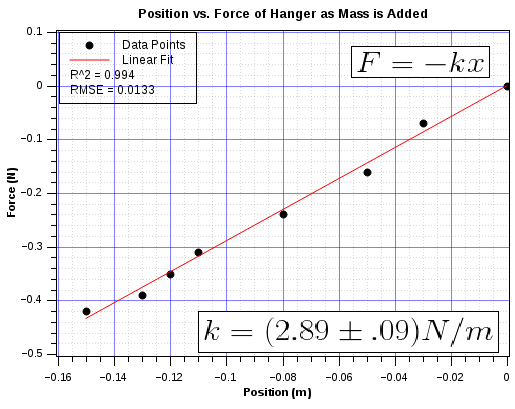
\includegraphics[width=\linewidth]{./Images/graph1a.png}
  \label{fig:graph_spring_const}
  \caption{Slope fit used to determine the spring constant $k$.}
  \end{center}
  \par\end{centering}
  \end{figure}

  \begin{align*}
  &\text{Spring Mass} 			&\text{\underline{46.39 g}} \\
  &\text{Hanging Mass} 			&\text{\underline{83.41 g}} \\
  &\text{Spring Constant} 		&\text{\underline{(2.89 $\pm$ .09) N/m}} \\
\end{align*}

\subsection*{\textbf{Part 1B: Simple Harmonic Motion}}
\begin{table}[h]
  \label{tb:data_period}
  \caption{Measuring the Period}
  \centering{}
  \begin{tabular}{|c|c|c|c|c|c|c|c|}
  \hline
  \textbf{}             & 1    & 2    & 3    & 4    & 5    & 6    & 7    \\ \hline
  \textbf{Time (sec)}   & 0.75 & 1.77 & 2.79 & 3.81 & 4.83 & 5.86 & 6.88 \\ \hline
  \textbf{Period (sec)} &      & 1.02 & 1.02 & 1.02 & 1.02 & 1.03 & 1.02 \\ \hline
  \end{tabular}
\end{table}

\begin{align*}
  &\text{Mass} 						&\text{\underline{129.80 g}} \\
  &\text{Spring Constant} 				&\text{\underline{2.972 N/m}} \\
  &\text{Average Period of Oscillation} 		&\text{\underline{1.02 sec}} \\
  &\text{Theoretical Period of Oscillation} 		&\text{\underline{1.16 sec}} \\
  &\text{Percent Error} 				&\text{\underline{-12\%}} \\
\end{align*}

\subsection*{\textbf{Part 2: Driven Harmonic Motion}}
\begin{table}[h]

  \label{tb:data_amp_freq}
  \caption{Amplitude vs. Frequency}

  \centering{}
  \begin{tabular}{|c|c|c|}
    \hline
    \textbf{Frequency (Hz)} & \textbf{\begin{tabular}[c]{@{}c@{}}Angular Frequency\\ $\omega$ (Hz)\end{tabular}} & \textbf{Amplitude (cm)} \\ \hline
    0.9            & 5.655             & 1.05      \\ \hline
    0.92           & 5.781             & 1.25      \\ \hline
    0.94           & 5.906             & 1.82      \\ \hline
    0.96           & 6.032             & 3.61      \\ \hline
    0.97           & 6.095             & 8.38      \\ \hline
    0.98           & 6.158             & 15        \\ \hline
    0.99           & 6.22              & 5.7       \\ \hline
    1.00           & 6.283             & 3.15      \\ \hline
    1.01           & 6.346             & 2.22      \\ \hline
    1.02           & 6.409             & 1.68      \\ \hline
    1.04           & 6.535             & 1.13      \\ \hline
    1.06           & 6.66              & 0.837     \\ \hline
  \end{tabular}
\end{table}
\begin{align*}
  &\text{Mass} 						&\text{\underline{55.3 g}} \\
  &\text{$\omega_0$ Measured} 				&\text{\underline{6.16 rad/s}} \\
  &\text{$\omega_0$ Theoretical} 			&\text{\underline{5.42 rad/s}} \\
\end{align*}
\begin{figure}[h!]
  \begin{centering}
  \begin{center}
  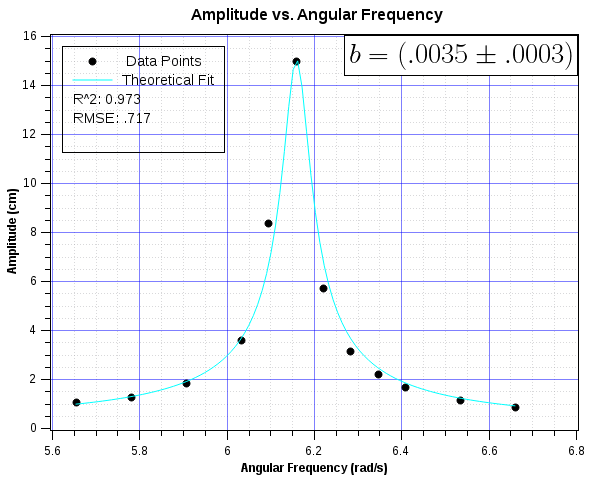
\includegraphics[width=\linewidth]{./Images/graph_amplitude_vw.png}
  \label{fig:graph_amplitude_vw}
  \caption{Graph of $A$ as a function of $\omega$}
  \end{center}
  \par\end{centering}
\end{figure}

\begin{figure}[h!]
  \begin{centering}
  \begin{center}
  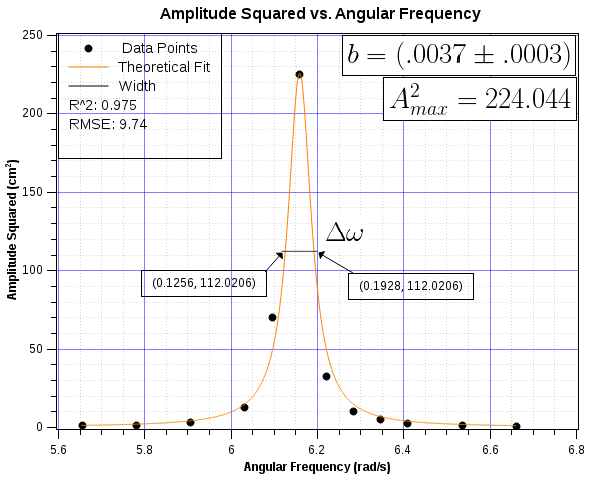
\includegraphics[width=\linewidth]{./Images/graph_amplitude_squared_vw.png}
  \label{fig:graph_amplitude_squared_vw}
  \caption{Graph of $A^2$ as a function of $\omega$}
  \end{center}
  \par\end{centering}
\end{figure}

\begin{figure}[h!]
  \begin{centering}
  \begin{center}
  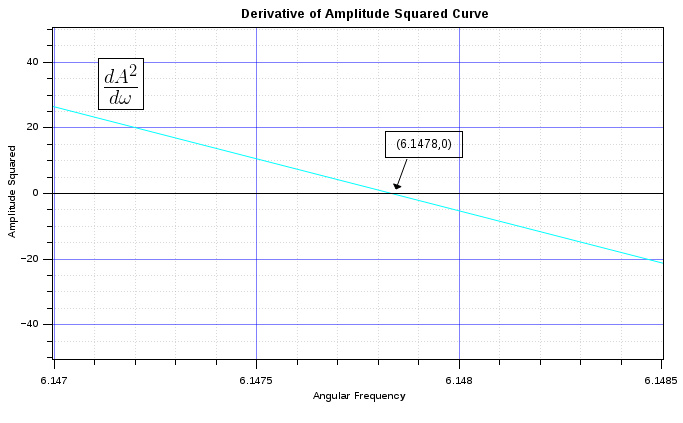
\includegraphics[width=\linewidth]{./Images/PlotDerivative.png}
  \label{fig:graph_deriv}
  \caption{Derivative of $A^2$, used to find $\omega_0$}
  \end{center}
  \par\end{centering}
\end{figure}


\begin{align*}
 &\text{Value for $b$:\footnotemark[1]} 		&\text{\underline{$3.5\times 10^{-3} (\pm 3\times 10^{-4})$}} \\
 &\text{Value for $b$:\footnotemark[2]} 		&\text{\underline{$3.7\times 10^{-3} (\pm 3\times 10^{-4})$}} \\
 &\text{Resonant Angular Frequency $\omega_0$}			&\text{\underline{$6.15$ rad/s}} \\
 &\text{Resonant Frequency $f_0$}				&\text{\underline{$.978$ Hz}} \\
 &\text{Width $\Delta \omega$} 					&\text{\underline{.0672 rad/s}} \\
 &\text{$Q$ (from $A^2$ vs. $\omega$ graph)} 			&\text{\underline{91.5}} \\
 &\text{Value for $b$ (From $Q$)} 				&\text{\underline{$5.13\times 10^{-3}$}} \\
 &\text{Percent difference in $b$\footnotemark[3]} 				&\text{\underline{37\%}} \\
\end{align*}
Notes:

[1]: From $A$ vs. $\omega$ graph.

[2]: From $A^2$ vs. $\omega$ graph.

[3]: Between values derived from $A^2$ vs. $\omega$ graph and from $Q$.

\textit{Taking into account experimental error, do the values of $b$ from the graph agree? Explain.}
The values for $b$ derived from the curve fit of both graphs agree, as both values are within each other's range of uncertainty. This was expected, as the $A^2$ graph is essentially a linear transformation of the data present in the $A$ vs $\omega$ graph. However, the value calculated from the quality factor differs significantly from both of these values. The difference in these values may stem from the nature of the curve fit, especially if the data was not taken at the exact resonance frequency and the fitting function yields an inaccurate maximum. The accuracy is also limited by using only several discrete data points, and also the additional uncertainty of the two other derived quantities used, $k$ and $\omega_0$. However, both calculations approximated $b$ to the same order of magnitude overall.
\section{Conclusion}
The results of this experiment yielded surprisingly accurate results, and led to a prediction for the system's resonant frequency that was even more accurate than the theoretical model used. Figures~\ref{fig:transcience} and~\ref{fig:resonance} show the wide distinction between the behavior of the spring-mass system when driven at frequencies that were within several radians of resonance and its behavior at resonance. Were one to observe the spring-mass system itself, the motion would appear chaotic or random, but interesting patterns in the wave function emerged as the frequencies approached resonance. For example, there were wider variations in the behavior of the transient "envelope" that shaped the overall amplitude of the graph over time, and several frequencies resulted in dense "nodes" of highly compacted oscillations over short periods of time that were themselves periodic. Furthermore, small perturbations in the system would result in remarkably large deviations from steady state behavior.

Further experiments in this area might involve prolonged data capture, on the order of hours or days, carried out in an isolated environment in order to investigate the extent to which transient solutions persist in an undisturbed system, and whether the steady-state solutions are dependent upon initial conditions. It was also found that increasing the instrument's data collection rate revealed smaller periodic variations in wave forms when the graphs zoomed in and examined in detail. As such, a higher level of instrument precision and resolution may also yield interesting results.

\begin{figure}[h!]
  \begin{centering}
  \begin{center}
  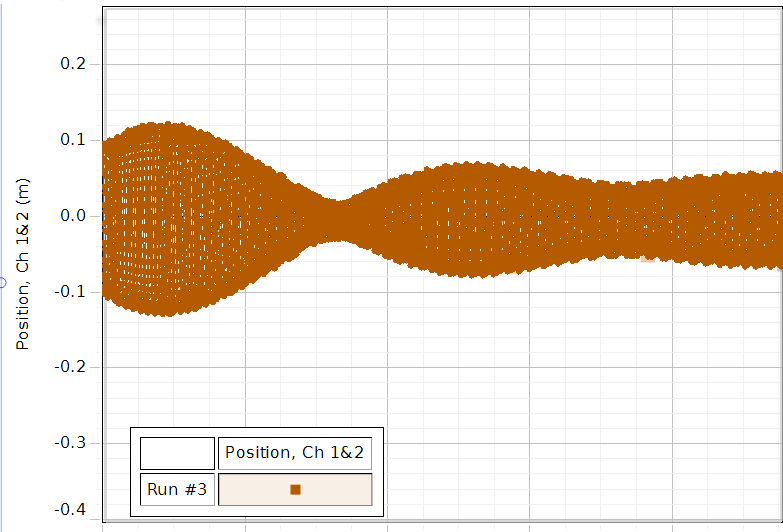
\includegraphics[width=\linewidth]{./Images/transcience.png}
  \label{fig:transcience}
  \caption{Transient behavior of frequencies far from resonance}
  \end{center}
  \par\end{centering}
  \end{figure}
\appendices{}

\begin{figure}[h!]
  \begin{centering}
  \begin{center}
  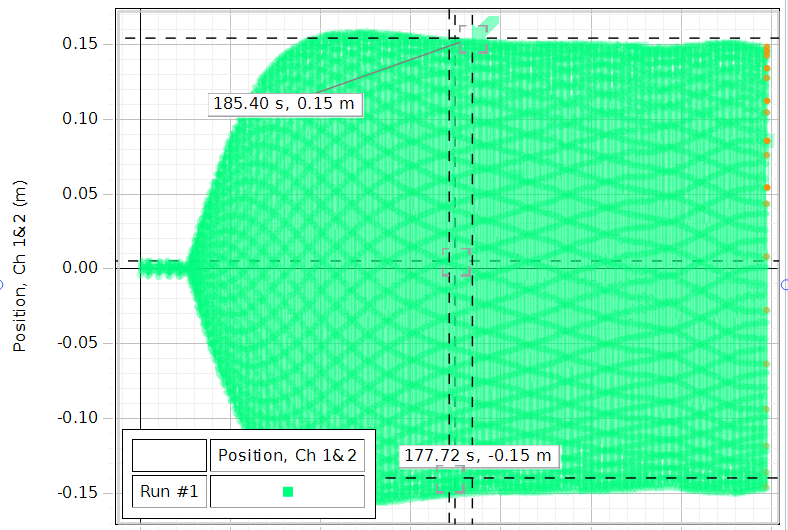
\includegraphics[width=\linewidth]{./Images/resonance.png}
  \label{fig:resonance}
  \caption{Resonant behavior}
  \end{center}
  \par\end{centering}
  \end{figure}
\appendices{}


\section{Derivation of Equation~\ref{eq:theoretical_period}}\label{append:period_deriv}

\begin{figure}[h!]
  \begin{centering}
  \begin{center}
  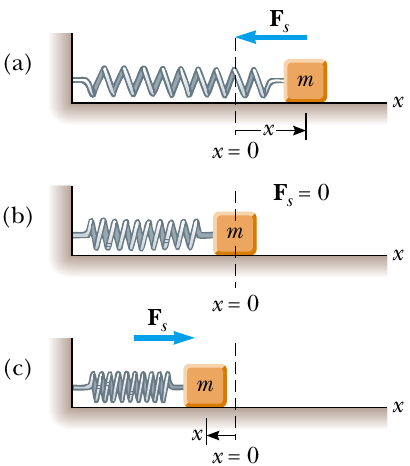
\includegraphics[width=\linewidth]{./Images/simple_pendulum.png}
  \caption{A Spring-Mass System}
  \label{fig:spring_mass}
  \end{center}
  \par\end{centering}
  \end{figure}

  In order to determine the period of the harmonic motion resulting in
  \textbf{Part 1}, consider the system depicted in Figure~\ref{fig:spring_mass}.
  The equilibrium position of the spring is denoted as the position $x=0$. It is known from Hooke's Law if the spring is stretched or compressed, it exerts a restoring force in proportion to its displacement from equilibrium. Thus the restoring force can be written as
  \begin{align*}
   \mathbf{F_S} = -k\mathbf{x}
  \end{align*}
  where $k$ is a physical constant associated with the spring, and the force is denoted as a negative quantity to signify that it tends to act in opposition to its displacement -- that is, the force always acts toward the equilibrium position.

  In the absence of friction, Newton's Second Law can be applied in the $x$ direction, resulting in the following second order differential equation:
  \begin{align*}
   \mathbf{F_S} &= m\mathbf{a_x} = -k \mathbf{x} \Rightarrow \\
   \mathbf{a_x} &= -\left(\frac{k}{m}\right)\mathbf{x} \Rightarrow \\
   \frac{d^2 x}{dt^2} &= -\left(\frac{k}{m}\right)\mathbf{x}
  \end{align*}
  To simplify solving this equation, let the ratio $k/m = \omega^2$. The equation of motion can now be rewritten as
  \begin{align}\label{eq:harmonic_eqn}
   \frac{d^2 x}{dt^2} = -\omega^2 x
  \end{align}
  The solutions to this equation must involve functions that are equal to the negative of their second derivatives. This suggests that sinusoidal waves with the quantity $\omega$ embedded within them would be potential solutions. One such solution is
  \begin{align}\label{eq:harmonic_soln}
   x(t) = Acos(\omega t + \phi)
  \end{align}
  Where $\phi$ is a phase constant that denotes the system's initial position. Taking the second derivative of $x$ with respect to $t$ results in
  \begin{align*}
   \frac{dx}{dt} &= -A\omega sin(\omega t + \phi) \\
   \frac{d^2x}{dt^2} &= -A \omega^2 cos(\omega t + \phi) \\
		    &= \omega^2 x
  \end{align*}
  which shows that Equation~\ref{eq:harmonic_soln} is a solution to Equation~\ref{eq:harmonic_eqn}.

  In order to examine the period of this motion, it is necessary to find the time required for the particle to go through one full cycle of its motion.

  Noting that trigonometric functions are periodic over an interval of $2\pi$, it follows that the phase $\omega t+\phi$ will be at the same value every time $\omega t$ increases by $2\pi$ radians. This results in the following relationship between the period $T$ and the phase:
  \begin{align*}
   (\omega(t+T) + \phi) &= 2\pi + (\omega t + \phi) \Rightarrow \\
   T &= \frac{2\pi}{\omega}
  \end{align*}
  Back-substituting using the fact that $\omega = \sqrt{k/m}$ gives a final expression for the period of the spring-mass system modeled by simple harmonic motion:
  \begin{equation}
   T = 2\pi \sqrt{\frac{m}{k}}
  \end{equation}

\section{Derivation of Equation~\ref{eq:theoretical_amplitude}}\label{append:amp_deriv}
 In the case of a driven damped harmonic oscillator, several more forces must be taken into account. If the driving force $F_{\text{ext}}$ varies periodically at a frequency $\omega$, then it can be expressed as
 \begin{align*}
  \mathbf{F_{\text{ext}}} = F_0 cos\omega t
 \end{align*}
 where $F_0$ is the amplitude of the driving force.

 Additionally, the presence of a damping force $\mathbf{R}$ such as air resistance or friction can be modeled linearly, where the magnitude of the force is proportional to the speed to the system's motion. The term for this force can then be written
 \begin{align*}
  \mathbf{R} = -b\mathbf{v} = -b\frac{dx}{dt}
 \end{align*}
 where $b$ is a physical constant that represents the damping coefficient and the magnitude is negative to denote that the force acts against the motion of the system.

 Taking into account the force of the spring $-kx$ and summing the forces according to Newton's Second Law yields
 \begin{gather*}
  \sum F = ma \Rightarrow \\
  F_0 cos(\omega t) - b \frac{dx}{dt} - kx = m\frac{d^2x}{dt^2} \Rightarrow \\
  \frac{d^2x}{dt^2}+ \left(\frac{b}{m}\right) \frac{dx}{dt} + \left(\frac{k}{m}\right)x = \left(\frac{F_0}{m}\right) cos(\omega t)
 \end{gather*}

  To simplify the equation, let $F_0cos(\omega t) = Fe^{i\omega t}$. From Euler's formula, $e^{ix} = cosx + isinx$, the original driving force is equal to the real portion of the complex exponential. Finding a solution to this equation now only requires a function that is equal to its first and second derivatives, and since exponentials have this property, we try a solution of the form
  \begin{align*}
   x(t) = Ae^{i(\omega t + \phi)}
  \end{align*}
  where $\phi$ is some phase difference between the driving force and the resulting motion. From this equation, the steady-state solution will be equal to the real portion of the exponential, and differentiating twice yields
  \begin{align*}
   -\omega^2 Ae^{i(\omega t + \phi)} + \frac{ib\omega}{m}Ae^{i(\omega t + \phi)} + \frac{k}{m}Ae^{i(\omega t + \phi)} = \frac{F_0}{m}Ae^{i\omega t}
  \end{align*}
  Factoring $e^{i\omega t}$ from both sides results in
  \begin{align*}
   -A\omega^2e^{i\phi}+A\frac{ib\omega}{m}e^{i\phi} + \frac{h}{m}e^{i\phi} = \frac{F_0}{m}
  \end{align*}
  Multiplying both sides by $e^{-i\phi}$ and factoring $A$ from the l.h.s.,
  \begin{align*}
    A\left(-\omega^2+\frac{ib\omega}{m} + \frac{h}{m}\right) = \frac{F_0}{m}e^{-i\phi}
  \end{align*}
  and solving for $A$,
  \begin{align}\label{eq:showing-a}
   A = \frac{(F_0/m)e^{-i\phi}}{-\omega^2+\frac{ib\omega}{m} + \frac{h}{m}}
  \end{align}
  Examining the denominator shows that the term can be represented as a complex number in the form of $a + ib$, where $a = -\omega^2 + \frac{k}{m}$ and $b = \frac{b\omega}{m}$. Since this can be represented in the polar form $\mathbf{r}e^{i\theta}$, it would be convenient to express the quantity given above in terms of its norm $\mathbf{r}$ and phase angle $\theta$. Figure~\ref{fig:real_im} shows this quantity plotted in the complex plane.
  \begin{figure}[h!]
  \begin{centering}
  \begin{center}
  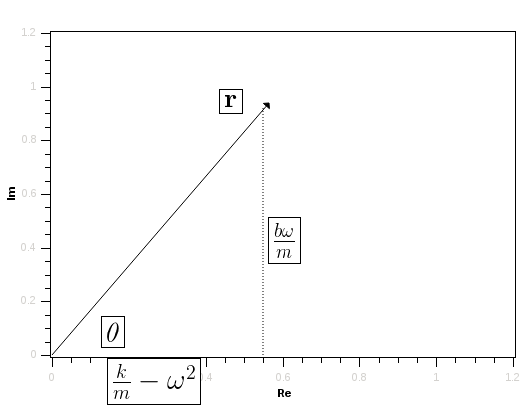
\includegraphics[width=\linewidth]{./Images/real_im.png}
  \caption{Denominator graphed in the }
  \label{fig:real_im}
  \end{center}
  \par\end{centering}
  \end{figure}

  Applying the Pythagorean theorem to the above triangle, we get
  \begin{align*}
   \mathbf{r} = \sqrt{(-\omega^2 + \frac{k}{m})^2 + (\frac{b\omega}{m})^2}
  \end{align*}
  and
  \begin{align*}
   \theta = tan^{-1}\left( \frac{b\omega/w}{(k/m) - \omega^2}\right)
  \end{align*}
  Letting the denominator in Equation~\ref{eq:showing-a}$= \mathbf{r}e^{i\theta}$ gives
  \begin{align*}
   A = \frac{(F_0/m)e^{-i\phi}}{\left(\sqrt{(-\omega^2 + \frac{k}{m})^2 + (\frac{b\omega}{m})^2}\right)e^{i\theta}}
  \end{align*}

  Because it is known that $A$ is a strictly real quantity, all of the complex components must cancel. From this, we conclude that
  \begin{align*}
   \frac{e^{-i\phi}}{e^{i\theta}} = 1 \Rightarrow \phi = -\theta
  \end{align*}
  and finally, letting $k/m = \omega_0^2$, gives the form of the equation used in the Theory section,
  \begin{align*}
   A = \frac{F_0/m}{\sqrt{(\omega_0^2 - \omega^2)^2 + (\frac{b\omega}{m})^2}}
  \end{align*}

%\bibliographystyle{plain}
%\bibliography{physbib}

\end{document}